% ----------------------------------------------------------------------------------------------------- %
% Manual da Classe UFTeX
% 
% Versão 2.1:   Março 2018
%
% Criado por:   Tiago da Silva Almeida
% Revisado por: Tiago da Silva Almeida
%               Rafael Lima de Carvalho
%               Ary Henrique Morais de Oliveira
%
% https://almeidatiago.github.io/uftex/
% ----------------------------------------------------------------------------------------------------- %

\documentclass[report]{uftex}
% ---- Esse comando cria o nome uftex estilizado
\newcommand\uftex{UF\TeX}

\usepackage{lipsum}
\usepackage{tikz}
\usepackage[siunitx]{circuitikz}
\usetikzlibrary{arrows}

\usepackage[alf,abnt-emphasize=bf]{abntex2cite}
\renewcommand{\backrefpagesname}{}
\renewcommand{\backref}{}
\renewcommand*{\backrefalt}[4]{}
% ----  Esse comandos são necessário no pré-ambulo para a impressão da lista de lista abreviatuas e de símbolos
\makelosymbols
\makeloabbreviations
% ---- Início do documento
\begin{document}
  % ---- Descrição do título do trabalho 
  \title{Análise empírica de algoritmos de ordenação}
  % ---- Nome do autor ou autores do trabalho
  \author{Yuri}{de Sousa Nascimento}
  \class{Projeto e análise de algoritmos}
  % ---- Nome do orientador do trabalho. O último campo representa o título do professor
  \advisor{Prof.}{Tiago}{da Silva Almeida}{Me.}
  % ---- Departamento representa o curso ao qual o trabalho está sendo apresentado. Descrito por meio de duas iniciais do curso
  \department{CC}
  % ---- Data da apresentação do trabalho
  \date{24}{05}{2023}
  % ---- Palavras-chaves em inglês do trabalho
  \foreignkeyword{\LaTeX}
  \foreignkeyword{\uftex}
  \foreignkeyword{Bachelor Thesis}
  \foreignkeyword{Scientific Writing}
  \foreignkeyword{University Extension}
  % ---- Comando responsável por criar a capa do trabalho e/ou folha de resto conforme a configuração exigida
  \maketitle

  \frontmatter
  
  \printlosymbols  
  \printloabbreviations
  % ---- Cria a lista de figuras. OPCIONAL
  %\listoffigures
  % ---- Cria a lista de tabelas. OPCIONAL
  %\listoftables 
  % ---- Cria o sumário. OBRIGATÓRIO
  \tableofcontents % sumário
% --- Marca o inicio dos elementos textuais. Capítulos.
\mainmatter
% ---- Defino o espaçamento de um e meio centímetros
\onehalfspacing
% ----------------------------------------------------------------------------------------------------- %
% Capítulos do trabalho
% ----------------------------------------------------------------------------------------------------- %
\ChapterStart{first}{First chapter}
\chapter{Introdução}

Conforme Cormen, um algoritmo é qualquer procedimento computacional bem definido que recebe algum valor, ou um conjunto de valores, como sua entrada e produz algum valor, ou um conjunto de valores, como sua saída, em uma quantidade finita de tempo.\\

Uma instância de um problema consiste de uma entrada – tal que ela satisfaça as restrições impostas pelo problema – necessária para computar a solução do problema.\\

Diferentes algoritmos criados para solucionar o mesmo problema geralmente diferem drasticamente quanto às suas eficiências. Nesse sentido, o problema analisado, no presente trabalho, refere ao problema de ordenação. Onde, dada uma entrada contendo uma sequência de $n$ números $\{a_1,a_2,...,a_n\}$, temos, como saída, a sequência $\{a_1 \leq a_2 \leq a_3 ... \leq a_n\}$. Desse modo, para determinar se um algoritmo é mais eficiente que outro, pode-se usar de duas abordagem:
\begin{itemize}
    \item Análise empírica: comparação entre os programas.
    \item Análise matemática: estudo das propriedades do algoritmo.
\end{itemize}

No presente relatório será abordado a análise empírica, sendo que ela avalia o custo/complexidade de um algoritmo a partir da avaliação da execução dele, quando implementado. Por meio dessa análise, pode-se:
\begin{itemize}
    \item avaliar o desempenho em uma determinada configuração de computador/linguagem.
    \item comparar computadores
    \item comparar linguagens
\end{itemize}

Apesar de algumas vantagens, a análise empírica tem suas desvantagens, como, por exemplo, se o programa for rodado várias vezes com a mesma instância, o tempo de execução necessário para processar tal instância pode variar. Além disso, para algumas instâncias, limitações de hardware podem limitar a análise.

\chapter{Métodos}


\section{Análise}
Para realizar as análises empíricas dos algoritmos de ordenação, os seguintes algoritmos foram implementados na linguagem C. Foram eles bubblesort, gnomesort, heapsort, insertionsort, mergesort, quicksort, selectionsort, shellsort, e timsort. Para analisar tais algoritmos, foi-se passado para cada um deles uma instância contendo elementos em ordem aleatória, crescente e decrescente tal que essas instância possuíam $1\times10^{3}, 1\times10^{4}, \{1,2,...,8,9\}\times10^{5}$ e $1\times10^{6}$ elementos. Para medir e comparar a eficiência do processamento dos algoritmos para as diferentes instâncias passadas, foi-se contabilizado a quantidade de comparações e trocas que cada algoritmo realizou, bem como o tempo de execução necessário para ordenar a instância.


\section{Hardware usado}
Para a realização da análise empírica, os algoritmos foram executados em uma máquina contendo as seguintes especificações:
\begin{itemize}
    \item CPU: Ryzen 3 2200G de 3.6 Ghz, quad core
    \item GPU: AMD Radeon RX 570, 4G
    \item RAM: HyperX 8GB 2666mhz, DDR4
\end{itemize}


\chapter{IMPLEMENTAÇÕES DOS ALGORITMOS}

\section{Bubblesort}
O algoritmo $Bubblesort$ trabalha de forma a movimentar, uma posição por vez, o maior valor existente na porção não ordenada de um array para a sua respectiva posição no array ordenado. Isso é repetido até que todos os elementos estejam nas suas posições correspondentes.\\

\begin{lstlisting}[language=C]
void bubblesort(long int* vet, size_t n){

    for(long int i = 0; i < n; ++i){
        for(long int j = n-1; j > i; --j){
            ++comp;
            if(vet[j-1] > vet[j]){
                exchange(&vet[j], &vet[j-1]);
                ++troca;
            }
        }
    }
}
}
\end{lstlisting}


\section{Gnomesort}

O algoritmo $Gnomesort$ é uma variação do insertionsort que não usa loops anhinhados. A ideia desse algoritmo é verificar os elementos $i$ e $i+1$ e, se eles estiverem na ordem correta, verificar os elementos seguintes; caso o os elementos não estejam na ordem correta, trocar $i+1$ com elementos anteriores até que ele esteje na posição correta.\\

\begin{lstlisting}[language=C]
void gnomesort(long int *vet, size_t n){
    long int index = 0;
  
    while(index < n){
        ++comp;
        if(index == 0)
            index++;
        if(vet[index -1] <= vet[index])
            index++;
        else{
            exchange(&vet[index], &vet[index -1]);
            index--;
            ++troca;
        }
    }
}
\end{lstlisting}


\section{Heapsort}
O algoritmo $Heapsort$ simula uma árvore binária completa (exceção do último nível) a partir de um array. Cada posição i do array passa a ser considerada o pai de duas outras posições, chamadas filhos: (2i + 1) e (2i + 2). Em seguida, o algoritmo reorganiza o array para que o pai seja sempre maior que os dois filhos. Ao fim desse processo, o elemento que é pai de todos é também o maior elemento do array. Este elemento poderá ser removido do heap e colocado na última posição do array e esse processo continua para o restante do heap/array.\\

\begin{lstlisting}[language=C]
void build_heap(long int* vet, size_t pai, size_t fim){
    long int aux = vet[pai];
    long int filho = 2 * pai + 1;

    while(filho <= fim){
        if(filho < fim){
            if(vet[filho] < vet[filho +1]){
                ++filho;
            }
        }

        ++comp;
        if(aux < vet[filho]){
            vet[pai] = vet[filho];
            pai = filho;
            filho = 2 * pai +1;
            ++troca;
        }else{
            filho = fim +1;
        }
    }
    vet[pai] = aux;
}

void heapsort(long int* vet, size_t size){
    for(long int i = (size-1)/2; i >= 0; --i){
        build_heap(vet, i, size-1);
    }
    for(long int i = size-1; i >= 1; --i){
        exchange(&vet[0], &vet[i]);
        build_heap(vet, 0, i-1);
    }
}
\end{lstlisting}


\section{Insertionsort}
O algoritmo $Insertionsort$ percorre um array e, para cada posição X, verifica se o seu valor está na posição correta. Isso é feito andando para o começo do array a partir da posição X e movimentando uma posição para frente os valores que são maiores do que o valor da posição X. Desse modo, teremos uma posição livre para inserir o valor da posição X em seu devido lugar.\\

\begin{lstlisting}[language=C]
void insertionsort(long int* vet, long int left, long int right){
   for (size_t i = left+1; i < right; i++){
      long int key = vet[i];
      long int j = i -1;
      ++comp;
      while(j >= left && key < vet[j]){
         vet[j+1] = vet[j];
         --j;
         ++troca;
      }
      vet[j+1] = key;
   }
}
\end{lstlisting}


\section{Mergesort}
O algoritmo $Mergesort$ divide, recursivamente, o array em duas partes até que cada posição dele seja considerada como um array de um único elemento. Em seguida, o algoritmo combina dois arrays de forma a obter um array maior e ordenado. Essa combinação dos arrays é feita intercalando seus elementos de acordo com o sentido da ordenação (crescente ou decrescente). Esse processo se repete até que exista apenas um array.\\

\begin{lstlisting}[language=C]
void merge(long int* vet, long int l, long int m, long int r){
   long int len1 = m -l +1, len2 = r -m;
   long int left[len1], right[len2];

   for (size_t i = 0; i < len1; i++)
      left[i] = vet[l + i]; // Filling left array
   for (size_t i = 0; i < len2; i++)
      right[i] = vet[m +1 +i]; // Filling right array

   size_t i = 0;
   size_t j = 0;
   size_t k = l;
   while (i < len1 && j < len2){ // Iterate into both arrays left and right{
   	++comp;
      if (left[i] <= right[j]){ // IF element in left is less then increment i by pushing into larger array{
         vet[k] = left[i];
         i++;
      } else {
         vet[k] = right[j]; // Element in right array is greater
         j++;
         ++troca;
      }
      k++;
   }
   while (i < len1){ // This loop copies remaining element in left array{
      vet[k] = left[i];
      k++;
      i++;
   }
   while (j < len2){ // This loop copies remaining element in right array{
      vet[k] = right[j];
      k++;
      j++;
   }
}

void mergesort(long int* vet, size_t inicio, size_t fim){

	if(inicio < fim){
		size_t meio = (inicio+fim)/2;
		mergesort(vet, inicio, meio);
		mergesort(vet, meio+1, fim);
		merge(vet, inicio, meio, fim);
	}
}
\end{lstlisting}


\section{Quicksort}
O algoritmo $Quicksort$, primeiramente, rearranja os valores de array de modo que os valores menores que o valor do pivô fiquem na parte esquerda do array, enquanto os valores maiores que o pivô ficam na parte direita. Supondo um array de tamanho N e que o pivô esteja na posição X, esse processo cria duas partições: [0, ..., X – 1] e [X + 1, ..., N – 1]. Em seguida, o algoritmo é aplicado recursivamente a cada partição. Esse processo se repete até que cada partição contenha um único elemento.\\

\begin{lstlisting}[language=C]
long int partition(long int* vet, long int inicio, long int final){
    long int key = vet[final], iterador = inicio -1;

    for(long int j = inicio; j < final; ++j){
        ++comp;
        if(vet[j] < key){
            ++iterador;
            exchange(&vet[iterador], &vet[j]);
            ++troca;
        }
    }
    exchange(&vet[iterador+1], &vet[final]);
    ++troca;
    return iterador +1;
}


void quicksort(long int* vet, long int inicio, long int fim){
    if(inicio < fim){
        long int pivo = partition(vet, inicio, fim);
        quicksort(vet, inicio, pivo -1);
        quicksort(vet, pivo +1, fim);
    }
}
\end{lstlisting}


\section{Selectionsort}
O algoritmo $Selectionsort$ divide o array em duas partes: a parte ordenada, à esquerda do elemento analisado, e a parte que ainda não foi ordenada, à direita do elemento. Para cada elemento do array, começando do primeiro, o algoritmo procura na parte não ordenada (direita) o menor valor (ordenação crescente) e troca os dois valores de lugar. Em seguida, o algoritmo avança para a próxima posição do array e repete esse processo. Isso é feito até que todo o array esteja ordenado.\\

\begin{lstlisting}[language=C]
void selectionsort(long int* vet, size_t n){
    
    for(size_t i = 0; i < n-1; ++i){
        size_t menor = i;

        for(size_t j = i+1; j < n; ++j){
            ++comp;
            if(vet[j] < vet[menor]){
                menor = j;
            }
        }

        if(i != menor){
            exchange(&vet[i], &vet[menor]);
            ++troca;
        }
    }   
}
\end{lstlisting}


\section{Shellsort}
O $Shellsort$ é uma otimização do insertionsort que permite a troca de elementos que estão distantes. A ideia é ordenar a lista de elementos para que, iniciando em qualquer lugar, tomando uma quantidade h de elemetentos, ela seja ordenada; tal que essa quantidade h de elementos é chamada de h-ardenada.\\

\begin{lstlisting}[language=C]
void shellsort(long int* vet, size_t n){
    for (long int gap = n/2; gap > 0; gap /= 2)
    {
        for (size_t i = gap; i < n; i += 1)
        {
            long int temp = vet[i];
            ++comp;
            long int j;
            for (j = i; j >= gap && vet[j -gap] > temp; j -= gap){
                vet[j] = vet[j -gap];
                ++troca;
            }
            vet[j] = temp;
        }
    }
}
\end{lstlisting}


\section{Timsort}
O $Timsort$ é um algoritmo de ordenação baseado nos algoritmos Insertion e Merge sort. A ideia é dividir o vetor em blocos chamados de RUN, ordenar esses blocos, um por um, usando o Insertionsort e, então, unir esses blocos usando a função Merge, do Mergesort. Se o tamanho do vetor for menor que o tamanho de um bloco RUN, então ele é ordenado usando o Insertionsort.\\

\begin{lstlisting}[language=C]
const int RUN = 32;
void timsort(long int* vet, size_t n){
    for (size_t i=0; i < n; i+=RUN)
        insertionsort(vet, i, min((i+31), n)); //Call insertionSort()

    for (size_t s = RUN; s < n; s = 2*s){
        for (size_t left = 0; left < n; left += 2*s){
            long int mid = left + s - 1; 
            long int right = min((left + 2*s - 1), (n-1));
            if(mid < right)
                merge(vet, left, mid, right); // merge sub array
        }
    }
}
\end{lstlisting}


\chapter{RESULTADOS}
A seguir são apresentadas tabelas que mostram o comportamento dos algoritmos para instâncias aleatória, crescente e decrescente, com quantidade de elementos de $1\times10^{3}, 1\times10^{4}, \{1,2,...,8,9\}\times10^{5}$ e $1\times10^{6}$. \\ 

\section{Tabelas}

\begin{table}[h!]
    \centering
    \begin{tabularx}{0.8\textwidth} {
  | >{\raggedright\arraybackslash}X 
  | >{\centering\arraybackslash}X 
  | >{\raggedleft\arraybackslash}X
  | >{\centering\arraybackslash}X |}
 \hline
 n   &   Tempo(seg)   &   Comparações     &    Trocas    \\
\hline
1000 & 0.005514 & 499500 & 249185   \\
\hline
10000 & 0.300751 & 49995000 & 24975864  \\
\hline
100000 & 32.723894 & 4999950000 & 2503447952    \\
\hline
200000 & 171.666300 & 19999900000 & 9972990404  \\
\hline
300000 & 388.640345 & 44999850000 & 22450657498 \\
\hline
400000 & 686.498350 & 79999800000 & 40027774620 \\
\hline
500000 & 1059.212025 & 124999750000 & 62394784027   \\
\hline
600000 & 1522.274723 & 179999700000 & 90007121038   \\
\hline
700000 & 2107.295848 & 244999650000 & 122787869370  \\
\hline
800000 & 2764.840854 & 319999600000 & 159986677534  \\
\hline
900000 & 3542.099250 & 404999550000 & 202396643276  \\
\hline
1000000 & 4391.192904 & 499999500000 & 250053898107 \\
\hline
\end{tabularx}
\caption{Bubblesort, aleatório}
\end{table}

\begin{table}[h!]
    \centering
    \begin{tabularx}{0.8\textwidth} {
  | >{\raggedright\arraybackslash}X 
  | >{\centering\arraybackslash}X 
  | >{\raggedleft\arraybackslash}X
  | >{\centering\arraybackslash}X |}
\hline
n   &   Tempo(seg)   &   Comparações     &    Trocas    \\
\hline
1000 & 0.002989 & 499500 & 0  \\
\hline
10000 & 0.092450 & 49995000 & 0  \\
\hline
100000 & 8.651060 & 4999950000 & 0  \\
\hline
200000 & 33.401417 & 19999900000 & 0  \\
\hline
300000 & 79.523717 & 44999850000 & 0  \\
\hline
400000 & 139.712857 & 79999800000 & 0  \\
\hline
500000 & 231.353135 & 124999750000 & 0  \\
\hline
600000 & 450.526261 & 179999700000 & 0  \\
\hline
700000 & 612.281525 & 244999650000 & 0  \\
\hline
800000 & 802.528626 & 319999600000 & 0  \\
\hline
900000 & 1012.964044 & 404999550000 & 0  \\
\hline
1000000 & 1252.151656 & 499999500000 & 0  \\
\hline
\end{tabularx}
\caption{Bubblesort, crescente}
\end{table}

\begin{table}[h!]
    \centering
    \begin{tabularx}{0.8\textwidth} {
  | >{\raggedright\arraybackslash}X 
  | >{\centering\arraybackslash}X 
  | >{\raggedleft\arraybackslash}X
  | >{\centering\arraybackslash}X |}
\hline
n   &   Tempo(seg)   &   Comparações     &    Trocas    \\
\hline
1000 & 0.007090 & 499500 & 499500  \\
\hline
10000 & 0.306663 & 49995000 & 49995000  \\
\hline
100000 & 47.558374 & 4999950000 & 4999950000  \\
\hline
200000 & 193.932538 & 19999900000 & 19999900000  \\
\hline
300000 & 309.478123 & 44999850000 & 44999850000  \\
\hline
400000 & 494.990543 & 79999800000 & 79999800000  \\
\hline
500000 & 1144.230130 & 124999750000 & 124999750000  \\
\hline
600000 & 1749.233020 & 179999700000 & 179999700000  \\
\hline
700000 & 1987.995923 & 244999650000 & 244999650000  \\
\hline
800000 & 3003.158171 & 319999600000 & 319999600000  \\
\hline
900000 & 3809.207139 & 404999550000 & 404999550000  \\
\hline
1000000 & 4583.418876 & 499999500000 & 499999500000  \\
\hline
\end{tabularx}
\caption{Bubblesort, decrescente}
\end{table}

% \section{Gnomesort}
\begin{table}[h!]
    \centering
    \begin{tabularx}{0.8\textwidth} {
  | >{\raggedright\arraybackslash}X 
  | >{\centering\arraybackslash}X 
  | >{\raggedleft\arraybackslash}X
  | >{\centering\arraybackslash}X |}
 \hline
 n   &   Tempo(seg)   &   Comparações     &    Trocas    \\
\hline
1000 &  0.002500 & 499361 & 249185 \\
\hline
10000 &  0.207900 & 49961718 & 24975864 \\
\hline
100000 &  30.618306 & 5006995894 & 2503447952 \\
\hline
200000 &  105.114902 & 19946180791 & 9972990404 \\
\hline
300000 &  242.197568 & 44901614983 & 22450657498 \\
\hline
400000 &  437.111799 & 80055949229 & 40027774620 \\
\hline
500000 &  619.277228 & 124790068042 & 62394784027 \\
\hline
600000 &  955.060298 & 180014842066 & 90007121038 \\
\hline
700000 &  1313.222865 & 245576438724 & 122787869370 \\
\hline
800000 &  1791.881784 & 319974155056 & 159986677534 \\
\hline
900000 &  2278.671625 & 404794186537 & 202396643276 \\
\hline
1000000 &  2900.027902 & 500108796201 & 250053898107 \\
\hline
\end{tabularx}
\caption{Gnomesort, aleatório}
\end{table}

\begin{table}[h!]
    \centering
    \begin{tabularx}{0.8\textwidth} {
  | >{\raggedright\arraybackslash}X 
  | >{\centering\arraybackslash}X 
  | >{\raggedleft\arraybackslash}X
  | >{\centering\arraybackslash}X |}
 \hline
 n   &   Tempo(seg)   &   Comparações     &    Trocas    \\
\hline
1000 & 0.000009 & 999 & 0  \\
\hline
10000 & 0.000069 & 9999 & 0  \\
\hline
100000 & 0.000276 & 99999 & 0  \\
\hline
200000 & 0.000568 & 199999 & 0  \\
\hline
300000 & 0.000820 & 299999 & 0  \\
\hline
400000 & 0.001090 & 399999 & 0  \\
\hline
500000 & 0.001377 & 499999 & 0  \\
\hline
600000 & 0.001629 & 599999 & 0  \\
\hline
700000 & 0.001924 & 699999 & 0  \\
\hline
800000 & 0.002201 & 799999 & 0  \\
\hline
900000 & 0.002496 & 899999 & 0  \\
\hline
1000000 & 0.002726 & 999999 & 0  \\
\hline
\end{tabularx}
\caption{Gnomesort, crescente}
\end{table}

\begin{table}[h!]
    \centering
    \begin{tabularx}{0.8\textwidth} {
  | >{\raggedright\arraybackslash}X 
  | >{\centering\arraybackslash}X 
  | >{\raggedleft\arraybackslash}X
  | >{\centering\arraybackslash}X |}
 \hline
 n   &   Tempo(seg)   &   Comparações     &    Trocas    \\
\hline
1000 & 0.010468 & 999000 & 499500  \\
\hline
10000 & 0.446132 & 99990000 & 49995000  \\
\hline
100000 & 42.932450 & 9999900000 & 4999950000  \\
\hline
200000 & 215.838401 & 39999800000 & 19999900000  \\
\hline
300000 & 551.661895 & 89999700000 & 44999850000  \\
\hline
400000 & 744.832737 & 159999600000 & 79999800000  \\
\hline
500000 & 1450.105700 & 249999500000 & 124999750000  \\
\hline
600000 & 1967.578099 & 359999400000 & 179999700000  \\
\hline
700000 & 2792.319604 & 489999300000 & 244999650000  \\
\hline
800000 & 3584.016330 & 639999200000 & 319999600000  \\
\hline
900000 & 4499.910007 & 809999100000 & 404999550000  \\
\hline
1000000 & 5588.802260 & 999999000000 & 499999500000  \\
\hline
\end{tabularx}
\caption{Gnomesort, decrescente}
\end{table}


% \section{Heapsort}
\begin{table}[h!]
    \centering
    \begin{tabularx}{0.8\textwidth} {
  | >{\raggedright\arraybackslash}X 
  | >{\centering\arraybackslash}X 
  | >{\raggedleft\arraybackslash}X
  | >{\centering\arraybackslash}X |}
 \hline
 n   &   Tempo(seg)   &   Comparações     &    Trocas    \\
\hline
1000 & 0.000200 & 8436 & 8102  \\
\hline
10000 & 0.002630 & 117623 & 114127  \\
\hline
100000 & 0.033956 & 1509883 & 1474971  \\
\hline
200000 & 0.042776 & 3219627 & 3149996  \\
\hline
300000 & 0.069413 & 5000406 & 4896067  \\
\hline
400000 & 0.100111 & 6839212 & 6699222  \\
\hline
500000 & 0.130451 & 8698333 & 8523703  \\
\hline
600000 & 0.167227 & 10601458 & 10392393  \\
\hline
700000 & 0.203725 & 12532355 & 12287829  \\
\hline
800000 & 0.249984 & 14478935 & 14199590  \\
\hline
900000 & 0.277332 & 16434101 & 16120846  \\
\hline
1000000 & 0.318731 & 18397055 & 18048206 \\
\hline
\end{tabularx}
\caption{Heapsort, aleatório}
\end{table}

\begin{table}[h!]
    \centering
    \begin{tabularx}{0.8\textwidth} {
  | >{\raggedright\arraybackslash}X 
  | >{\centering\arraybackslash}X 
  | >{\raggedleft\arraybackslash}X
  | >{\centering\arraybackslash}X |}
 \hline
 n   &   Tempo(seg)   &   Comparações     &    Trocas    \\
\hline
1000 & 0.000236 & 8813 & 8709  \\
\hline
10000 & 0.002944 & 122288 & 121957  \\
\hline
100000 & 0.024257 & 1556441 & 1550855  \\
\hline
200000 & 0.029632 & 3313748 & 3299161  \\
\hline
300000 & 0.045399 & 5140727 & 5111161  \\
\hline
400000 & 0.061669 & 7031767 & 6983469  \\
\hline
500000 & 0.079243 & 8922789 & 8855701  \\
\hline
600000 & 0.096501 & 10884155 & 10828705  \\
\hline
700000 & 0.116497 & 12878903 & 12818735  \\
\hline
800000 & 0.133143 & 14873643 & 14808701  \\
\hline
900000 & 0.151755 & 16869595 & 16798193  \\
\hline
1000000 & 0.172521 & 18864660 & 18787793  \\
\hline
\end{tabularx}
\caption{Heapsort, crescente}
\end{table}

\begin{table}[h!]
    \centering
    \begin{tabularx}{0.8\textwidth} {
  | >{\raggedright\arraybackslash}X 
  | >{\centering\arraybackslash}X 
  | >{\raggedleft\arraybackslash}X
  | >{\centering\arraybackslash}X |}
 \hline
 n   &   Tempo(seg)   &   Comparações     &    Trocas    \\
\hline
1000 & 0.000223 & 7991 & 7317  \\
\hline
10000 & 0.002899 & 113360 & 106697  \\
\hline
100000 & 0.030072 & 1463377 & 1397435  \\
\hline
200000 & 0.029441 & 3128277 & 2995729  \\
\hline
300000 & 0.045526 & 4870499 & 4676247  \\
\hline
400000 & 0.062690 & 6659505 & 6410615  \\
\hline
500000 & 0.079769 & 8489282 & 8168451  \\
\hline
600000 & 0.115379 & 10354936 & 9956841  \\
\hline
700000 & 0.115745 & 12234832 & 11759605  \\
\hline
800000 & 0.135163 & 14132618 & 13584465  \\
\hline
900000 & 0.150760 & 16069055 & 15458795  \\
\hline
1000000 & 0.168636 & 18001491 & 17333409 \\
\hline
\end{tabularx}
\caption{Heapsort, decrescente}
\end{table}


% \section{Insertionsort}
\begin{table}[h!]
    \centering
    \begin{tabularx}{0.8\textwidth} {
  | >{\raggedright\arraybackslash}X 
  | >{\centering\arraybackslash}X 
  | >{\raggedleft\arraybackslash}X
  | >{\centering\arraybackslash}X |}
 \hline
 n   &   Tempo(seg)   &   Comparações     &    Trocas    \\
\hline
1000 & 0.000510 & 999 & 249185  \\
\hline
10000 & 0.050798 & 9999 & 24975864  \\
\hline
100000 & 6.067503 & 99999 & 2503447952  \\
\hline
200000 & 24.411696 & 199999 & 9972990404  \\
\hline
300000 & 55.154221 & 299999 & 22450657498  \\
\hline
400000 & 98.553641 & 399999 & 40027774620  \\
\hline
500000 & 154.346585 & 499999 & 62394784027  \\
\hline
600000 & 257.821471 & 599999 & 90007121038  \\
\hline
700000 & 306.128545 & 699999 & 122787869370  \\
\hline
800000 & 396.245174 & 799999 & 159986677534  \\
\hline
900000 & 552.124342 & 899999 & 202396643276  \\
\hline
1000000 & 600.033389 & 999999 & 250053898107 \\
\hline
\end{tabularx}
\caption{Insertionsort, aleatório}
\end{table}

\begin{table}[h!]
    \centering
    \begin{tabularx}{0.8\textwidth} {
  | >{\raggedright\arraybackslash}X 
  | >{\centering\arraybackslash}X 
  | >{\raggedleft\arraybackslash}X
  | >{\centering\arraybackslash}X |}
 \hline
 n   &   Tempo(seg)   &   Comparações     &    Trocas    \\
\hline
\hline
1000 & 0.000016 & 999 & 0  \\
\hline
10000 & 0.000094 & 9999 & 0  \\
\hline
100000 & 0.000235 & 99999 & 0  \\
\hline
200000 & 0.000492 & 199999 & 0  \\
\hline
300000 & 0.000677 & 299999 & 0  \\
\hline
400000 & 0.000958 & 399999 & 0  \\
\hline
500000 & 0.001218 & 499999 & 0  \\
\hline
600000 & 0.001588 & 599999 & 0  \\
\hline
700000 & 0.001750 & 699999 & 0  \\
\hline
800000 & 0.001960 & 799999 & 0  \\
\hline
900000 & 0.002236 & 899999 & 0  \\
\hline
1000000 & 0.002507 & 999999 & 0  \\
\hline
\end{tabularx}
\caption{Insertionsort, crescente}
\end{table}

\begin{table}[h!]
    \centering
    \begin{tabularx}{0.8\textwidth} {
  | >{\raggedright\arraybackslash}X 
  | >{\centering\arraybackslash}X 
  | >{\raggedleft\arraybackslash}X
  | >{\centering\arraybackslash}X |}
 \hline
 n   &   Tempo(seg)   &   Comparações     &    Trocas    \\
1000 & 0.003530 & 999 & 499500  \\
\hline
10000 & 0.096134 & 9999 & 49995000  \\
\hline
100000 & 9.011488 & 99999 & 4999950000  \\
\hline
200000 & 53.639241 & 199999 & 19999900000  \\
\hline
300000 & 141.065438 & 299999 & 44999850000  \\
\hline
400000 & 166.225205 & 399999 & 79999800000  \\
\hline
500000 & 258.234492 & 499999 & 124999750000  \\
\hline
600000 & 366.967374 & 599999 & 179999700000  \\
\hline
700000 & 906.812994 & 699999 & 244999650000  \\
\hline
800000 & 938.283282 & 799999 & 319999600000  \\
\hline
900000 & 991.555619 & 899999 & 404999550000  \\
\hline
1000000 & 1942.532041 & 999999 & 499999500000  \\
\hline
\end{tabularx}
\caption{Insertionsort, decrescente}
\end{table}


% \section{Mergesort}
\begin{table}[h!]
    \centering
    \begin{tabularx}{0.8\textwidth} {
  | >{\raggedright\arraybackslash}X 
  | >{\centering\arraybackslash}X 
  | >{\raggedleft\arraybackslash}X
  | >{\centering\arraybackslash}X |}
 \hline
 n   &   Tempo(seg)   &   Comparações     &    Trocas    \\
\hline
1000 & 0.000080 & 8711 & 4318  \\
\hline
10000 & 0.001012 & 120537 & 59244  \\
\hline
100000 & 0.011782 & 1536468 & 759889  \\
\hline
200000 & 0.025045 & 3272881 & 1620005  \\
\hline
300000 & 0.040071 & 5085014 & 2511101  \\
\hline
400000 & 0.052426 & 6945514 & 3439798  \\
\hline
500000 & 0.066677 & 8837110 & 4390212  \\
\hline
600000 & 0.080510 & 10769183 & 5320898  \\
\hline
700000 & 0.095935 & 12724655 & 6275876  \\
\hline
800000 & 0.109991 & 14691344 & 7279485  \\
\hline
900000 & 0.125090 & 16678608 & 8256186  \\
\hline
1000000 & 0.143499 & 18675006 & 9278929 \\
\hline
\end{tabularx}
\caption{Mergensort, aleatório}
\end{table}

\begin{table}[h!]
    \centering
    \begin{tabularx}{0.8\textwidth} {
  | >{\raggedright\arraybackslash}X 
  | >{\centering\arraybackslash}X 
  | >{\raggedleft\arraybackslash}X
  | >{\centering\arraybackslash}X |}
 \hline
 n   &   Tempo(seg)   &   Comparações     &    Trocas    \\
\hline
1000 & 0.000059 & 5044 & 0  \\
\hline
10000 & 0.000575 & 69008 & 0  \\
\hline
100000 & 0.006636 & 853904 & 0  \\
\hline
200000 & 0.014012 & 1807808 & 0  \\
\hline
300000 & 0.021336 & 2797264 & 0  \\
\hline
400000 & 0.028990 & 3815616 & 0  \\
\hline
500000 & 0.037257 & 4783216 & 0  \\
\hline
600000 & 0.044394 & 5894528 & 0  \\
\hline
700000 & 0.053678 & 7000336 & 0  \\
\hline
800000 & 0.061870 & 8031232 & 0  \\
\hline
900000 & 0.070271 & 9084240 & 0  \\
\hline
1000000 & 0.077618 & 10066432 & 0  \\
\hline
\end{tabularx}
\caption{Mergesort, crescente}
\end{table}

\begin{table}[h!]
    \centering
    \begin{tabularx}{0.8\textwidth} {
  | >{\raggedright\arraybackslash}X 
  | >{\centering\arraybackslash}X 
  | >{\raggedleft\arraybackslash}X
  | >{\centering\arraybackslash}X |}
 \hline
 n   &   Tempo(seg)   &   Comparações     &    Trocas    \\
\hline
1000 & 0.000048 & 4932 & 4932  \\
\hline
10000 & 0.000589 & 64608 & 64608  \\
\hline
100000 & 0.006806 & 815024 & 815024  \\
\hline
200000 & 0.033115 & 1730048 & 1730048  \\
\hline
300000 & 0.021871 & 2678448 & 2678448  \\
\hline
400000 & 0.029894 & 3660096 & 3660096  \\
\hline
500000 & 0.038579 & 4692496 & 4692496  \\
\hline
600000 & 0.047065 & 5656896 & 5656896  \\
\hline
700000 & 0.055464 & 6651088 & 6651088  \\
\hline
800000 & 0.063807 & 7720192 & 7720192  \\
\hline
900000 & 0.072123 & 8767184 & 8767184  \\
\hline
1000000 & 0.079721 & 9884992 & 9884992  \\
\hline
\end{tabularx}
\caption{Mergesort, decrescente}
\end{table}


% \section{Quicksort}
\begin{table}[h!]
    \centering
    \begin{tabularx}{0.8\textwidth} {
  | >{\raggedright\arraybackslash}X 
  | >{\centering\arraybackslash}X 
  | >{\raggedleft\arraybackslash}X
  | >{\centering\arraybackslash}X |}
 \hline
 n   &   Tempo(seg)   &   Comparações     &    Trocas    \\
\hline
1000 & 0.000232 & 10677 & 7336  \\
\hline
10000 & 0.002041 & 149364 & 83257  \\
\hline
100000 & 0.015794 & 2079900 & 1217010  \\
\hline
200000 & 0.040811 & 4254051 & 2359739  \\
\hline
300000 & 0.059895 & 7067680 & 3844969  \\
\hline
400000 & 0.075544 & 9101331 & 4980831  \\
\hline
500000 & 0.106553 & 11776390 & 6243400  \\
\hline
600000 & 0.145120 & 15101888 & 8285236  \\
\hline
700000 & 0.153213 & 16565377 & 8886213  \\
\hline
800000 & 0.192934 & 19728710 & 10399255  \\
\hline
900000 & 0.209007 & 21928147 & 11270308  \\
\hline
1000000 & 0.240464 & 23986050 & 13039846 \\
\hline
\end{tabularx}
\caption{Quicksort, aleatório}
\end{table}

\begin{table}[h!]
    \centering
    \begin{tabularx}{0.8\textwidth} {
  | >{\raggedright\arraybackslash}X 
  | >{\centering\arraybackslash}X 
  | >{\raggedleft\arraybackslash}X
  | >{\centering\arraybackslash}X |}
 \hline
 n   &   Tempo(seg)   &   Comparações     &    Trocas    \\
\hline
1000 & 0.005046 & 499500 & 500499  \\
\hline
10000 & 0.493096 & 49995000 & 50004999  \\
\hline
100000 & 51.733237 & 4999950000 & 5000049999  \\
\hline
\end{tabularx}
\caption{Quicksort, crescente}
\end{table}

\begin{table}[h!]
    \centering
    \begin{tabularx}{0.8\textwidth} {
  | >{\raggedright\arraybackslash}X 
  | >{\centering\arraybackslash}X 
  | >{\raggedleft\arraybackslash}X
  | >{\centering\arraybackslash}X |}
 \hline
 n   &   Tempo(seg)   &   Comparações     &    Trocas    \\
\hline
1000 & 0.005001 & 499500 & 250499  \\
\hline
10000 & 0.331269 & 49995000 & 25004999  \\
\hline
100000 & 31.296026 & 4999950000 & 2500049999  \\
\hline
20000 & 46.070497 & 7366469190 & 3683360147  \\
\hline
\end{tabularx}
\caption{Quicksort, decrescente}
\end{table}


% \section{Selectionsort}
\begin{table}[h!]
    \centering
    \begin{tabularx}{0.8\textwidth} {
  | >{\raggedright\arraybackslash}X 
  | >{\centering\arraybackslash}X 
  | >{\raggedleft\arraybackslash}X
  | >{\centering\arraybackslash}X |}
 \hline
 n   &   Tempo(seg)   &   Comparações     &    Trocas    \\
\hline
1000 & 0.002785 & 499500 & 991  \\
\hline
10000 & 0.114248 & 49995000 & 9992  \\
\hline
100000 & 11.261241 & 4999950000 & 99990  \\
\hline
200000 & 45.037807 & 19999900000 & 199984  \\
\hline
300000 & 101.247408 & 44999850000 & 299988  \\
\hline
400000 & 179.941800 & 79999800000 & 399980  \\
\hline
500000 & 281.443916 & 124999750000 & 499987  \\
\hline
600000 & 406.063803 & 179999700000 & 599995  \\
\hline
700000 & 554.224734 & 244999650000 & 699981  \\
\hline
800000 & 725.953637 & 319999600000 & 799993  \\
\hline
900000 & 922.778084 & 404999550000 & 899980  \\
\hline
1000000 & 1142.254526 & 499999500000 & 999981  \\
\hline
\end{tabularx}
\caption{Selectionsort, aleatório}
\end{table}

\begin{table}[h!]
    \centering
    \begin{tabularx}{0.8\textwidth} {
  | >{\raggedright\arraybackslash}X 
  | >{\centering\arraybackslash}X 
  | >{\raggedleft\arraybackslash}X
  | >{\centering\arraybackslash}X |}
 \hline
 n   &   Tempo(seg)   &   Comparações     &    Trocas    \\
\hline
1000 & 0.002846 & 499500 & 0  \\
\hline
10000 & 0.113849 & 49995000 & 0  \\
\hline
100000 & 11.256547 & 4999950000 & 0  \\
\hline
200000 & 45.009932 & 19999900000 & 0  \\
\hline
300000 & 101.462775 & 44999850000 & 0  \\
\hline
400000 & 180.911438 & 79999800000 & 0  \\
\hline
500000 & 282.873749 & 124999750000 & 0  \\
\hline
600000 & 409.004904 & 179999700000 & 0  \\
\hline
700000 & 557.167017 & 244999650000 & 0  \\
\hline
800000 & 727.749909 & 319999600000 & 0  \\
\hline
900000 & 918.501047 & 404999550000 & 0  \\
\hline
1000000 & 1135.334070 & 499999500000 & 0  \\
\hline
\end{tabularx}
\caption{Selectionsort, crescente}
\end{table}

\begin{table}[h!]
    \centering
    \begin{tabularx}{0.8\textwidth} {
  | >{\raggedright\arraybackslash}X 
  | >{\centering\arraybackslash}X 
  | >{\raggedleft\arraybackslash}X
  | >{\centering\arraybackslash}X |}
 \hline
 n   &   Tempo(seg)   &   Comparações     &    Trocas    \\
\hline
1000 & 0.001516 & 499500 & 500  \\
\hline
10000 & 0.135242 & 49995000 & 5000  \\
\hline
100000 & 11.587708 & 4999950000 & 50000  \\
\hline
200000 & 46.394593 & 19999900000 & 100000  \\
\hline
300000 & 104.351848 & 44999850000 & 150000  \\
\hline
400000 & 186.114453 & 79999800000 & 200000  \\
\hline
500000 & 293.186715 & 124999750000 & 250000  \\
\hline
600000 & 419.122492 & 179999700000 & 300000  \\
\hline
700000 & 573.336565 & 244999650000 & 350000  \\
\hline
800000 & 751.208892 & 319999600000 & 400000  \\
\hline
900000 & 951.649183 & 404999550000 & 450000  \\
\hline
1000000 & 1171.327412 & 499999500000 & 500000  \\
\hline
\end{tabularx}
\caption{Selectionsort, decrescente}
\end{table}


% \section{Shellsort}
\begin{table}[h!]
    \centering
    \begin{tabularx}{0.8\textwidth} {
  | >{\raggedright\arraybackslash}X 
  | >{\centering\arraybackslash}X 
  | >{\raggedleft\arraybackslash}X
  | >{\centering\arraybackslash}X |}
 \hline
 n   &   Tempo(seg)   &   Comparações     &    Trocas    \\
\hline
1000 & 0.000281 & 8006 & 6958  \\
\hline
10000 & 0.004266 & 120005 & 155236  \\
\hline
100000 & 0.042395 & 1500006 & 2792208  \\
\hline
200000 & 0.075192 & 3200006 & 6797940  \\
\hline
300000 & 0.103793 & 5100008 & 10661386  \\
\hline
400000 & 0.164657 & 6800006 & 17121153  \\
\hline
500000 & 0.207145 & 8500007 & 19950705  \\
\hline
600000 & 0.259706 & 10800008 & 24841577  \\
\hline
700000 & 0.265710 & 12600009 & 31646869  \\
\hline
800000 & 0.373621 & 14400006 & 38853061  \\
\hline
900000 & 0.393763 & 16200011 & 40634531  \\
\hline
1000000 & 0.422650 & 18000007 & 46859906  \\
\hline
\end{tabularx}
\caption{Shellsort, aleatório}
\end{table}

\begin{table}[h!]
    \centering
    \begin{tabularx}{0.8\textwidth} {
  | >{\raggedright\arraybackslash}X 
  | >{\centering\arraybackslash}X 
  | >{\raggedleft\arraybackslash}X
  | >{\centering\arraybackslash}X |}
 \hline
 n   &   Tempo(seg)   &   Comparações     &    Trocas    \\
\hline
1000 & 0.000077 & 8006 & 0  \\
\hline
10000 & 0.001130 & 120005 & 0  \\
\hline
100000 & 0.014297 & 1500006 & 0  \\
\hline
200000 & 0.030285 & 3200006 & 0  \\
\hline
300000 & 0.030838 & 5100008 & 0  \\
\hline
400000 & 0.046829 & 6800006 & 0  \\
\hline
500000 & 0.059074 & 8500007 & 0  \\
\hline
600000 & 0.074330 & 10800008 & 0  \\
\hline
700000 & 0.088945 & 12600009 & 0  \\
\hline
800000 & 0.101213 & 14400006 & 0  \\
\hline
900000 & 0.113399 & 16200011 & 0  \\
\hline
1000000 & 0.123279 & 18000007 & 0  \\
\hline
\end{tabularx}
\caption{Shellsort, crescente}
\end{table}

\begin{table}[h!]
    \centering
    \begin{tabularx}{0.8\textwidth} {
  | >{\raggedright\arraybackslash}X 
  | >{\centering\arraybackslash}X 
  | >{\raggedleft\arraybackslash}X
  | >{\centering\arraybackslash}X |}
 \hline
 n   &   Tempo(seg)   &   Comparações     &    Trocas    \\
\hline
1000 & 0.000084 & 8006 & 4700  \\
\hline
10000 & 0.001138 & 120005 & 62560  \\
\hline
100000 & 0.014434 & 1500006 & 844560  \\
\hline
200000 & 0.026136 & 3200006 & 1789120  \\
\hline
300000 & 0.043615 & 5100008 & 2500880  \\
\hline
400000 & 0.052759 & 6800006 & 3778240  \\
\hline
500000 & 0.070801 & 8500007 & 4428752  \\
\hline
600000 & 0.090154 & 10800008 & 5301760  \\
\hline
700000 & 0.106377 & 12600009 & 6413904  \\
\hline
800000 & 0.124701 & 14400006 & 7956480  \\
\hline
900000 & 0.139076 & 16200011 & 8207632  \\
\hline
1000000 & 0.154852 & 18000007 & 9357504  \\
\hline
\end{tabularx}
\caption{Shellsort, decrescente}
\end{table}


% \section{Timsort}
\begin{table}[h!]
    \centering
    \begin{tabularx}{0.8\textwidth} {
  | >{\raggedright\arraybackslash}X 
  | >{\centering\arraybackslash}X 
  | >{\raggedleft\arraybackslash}X
  | >{\centering\arraybackslash}X |}
 \hline
 n   &   Tempo(seg)   &   Comparações     &    Trocas    \\
\hline
1000 & 0.000210 & 5831 & 9541  \\
\hline
10000 & 0.002941 & 94677 & 111653  \\
\hline
100000 & 0.026297 & 1276955 & 1287282  \\
\hline
200000 & 0.035982 & 2753670 & 2673149  \\
\hline
300000 & 0.054198 & 4363683 & 4093668  \\
\hline
400000 & 0.073122 & 5907449 & 5543342  \\
\hline
500000 & 0.102139 & 7409614 & 7051012  \\
\hline
600000 & 0.124170 & 9327568 & 8494572  \\
\hline
700000 & 0.127660 & 10850869 & 9950926  \\
\hline
800000 & 0.163255 & 12614629 & 11494006  \\
\hline
900000 & 0.183983 & 14125065 & 13007155  \\
\hline
1000000 & 0.187233 & 15819188 & 14600667  \\
\hline
\hline
\end{tabularx}
\caption{Timsort, aleatório}
\end{table}

\begin{table}[h!]
    \centering
    \begin{tabularx}{0.8\textwidth} {
  | >{\raggedright\arraybackslash}X 
  | >{\centering\arraybackslash}X 
  | >{\raggedleft\arraybackslash}X
  | >{\centering\arraybackslash}X |}
 \hline
 n   &   Tempo(seg)   &   Comparações     &    Trocas    \\
\hline
1000 & 0.000090 & 3497 & 0  \\
\hline
10000 & 0.001367 & 56095 & 0  \\
\hline
100000 & 0.012788 & 721718 & 0  \\
\hline
200000 & 0.025227 & 1543436 & 0  \\
\hline
300000 & 0.030268 & 2464898 & 0  \\
\hline
400000 & 0.035690 & 3286872 & 0  \\
\hline
500000 & 0.045810 & 4016526 & 0  \\
\hline
600000 & 0.057688 & 5229796 & 0  \\
\hline
700000 & 0.069349 & 6019034 & 0  \\
\hline
800000 & 0.080581 & 6973744 & 0  \\
\hline
900000 & 0.089822 & 7696742 & 0  \\
\hline
1000000 & 0.106465 & 8533052 & 0  \\
\hline
\end{tabularx}
\caption{Timsort, crescente}
\end{table}

\begin{table}[h!]
    \centering
    \begin{tabularx}{0.8\textwidth} {
  | >{\raggedright\arraybackslash}X 
  | >{\centering\arraybackslash}X 
  | >{\raggedleft\arraybackslash}X
  | >{\centering\arraybackslash}X |}
 \hline
 n   &   Tempo(seg)   &   Comparações     &    Trocas    \\
\hline
1000 & 0.000194 & 3377 & 16883  \\
\hline
10000 & 0.002454 & 48991 & 184816  \\
\hline
100000 & 0.029697 & 658774 & 2018149  \\
\hline
200001 & 0.024875 & 1417554 & 4136304  \\
\hline
300000 & 0.046530 & 2209698 & 6287823  \\
\hline
400000 & 0.057458 & 3035096 & 8472596  \\
\hline
500000 & 0.065329 & 3911246 & 10708121  \\
\hline
600000 & 0.081208 & 4719396 & 12875646  \\
\hline
700000 & 0.112376 & 5557338 & 15072963  \\
\hline
800000 & 0.138323 & 6470192 & 17345192  \\
\hline
900000 & 0.135368 & 7360934 & 19595309  \\
\hline
1000000 & 0.167905 & 8322492 & 21916242  \\
\hline
\end{tabularx}
\caption{Timsort, decrescente}
\end{table}


\section{Gráficos}
A partir das tabelas anteriores, foram gerados os gráficos a seguir com o objetivo de comparar o comportamento dos algoritmos de forma visual. Desse modo, em cada gráfico, há o comportamento de todos os algoritmo para as devidas instâncias, que estão especificadas em cada gráfico. Deve-se deixar claro que, por conta das grandes diferenças de execução de algoritmos eficientes e não eficiente, alguns gráficos dão a impressão que certos algoritmos tiveram um comportamento costante, ficando apenas em 0 (zero).

\begin{figure}[h]
\centering
\caption{Aleatório, N x Tempo}
\includegraphics[width=0.8\textwidth]{graphs/aleatório-tempo.png}

Na Figura 1, os algoritmos que mais custaram para terminar de executar as grandes instâncias foram o bubble, insertion, selection e gnome. Os demais não levaram um pouco menos de 1 segundo de tempo, como se pode ver no gráfico.
\end{figure}


\begin{figure}[h]
\centering
\caption{Aleatório, N x Comparações}
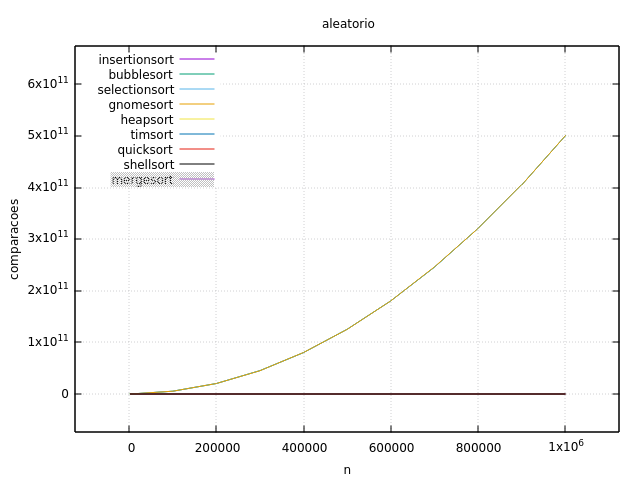
\includegraphics[width=0.8\textwidth]{graphs/aleatório-comparações.png}

Na figura 2, os algoritmos que mais realizaram comparações para processar um vetor disposto de forma aleatório foram o bubble, selection e gnome sort. Quanto aos demais algoritmos, eles tiveram uma quantidade significativa de comparações, mas não tanto como os três algoritmos citados.
\end{figure}

\begin{figure}[h]
\centering
\caption{Aleatório, N x Trocas}
\includegraphics[width=0.8\textwidth]{graphs/aleatório-trocas.png}

Como mostra a Figura 3, os algoritmos que mais realizaram trocas para ordenar um vertor com os elementos desordenados aleatoriamente foram o insertion e bubble sortl. Porém, diferente do que o gráfico mostra, os demais algoritmos tiveram uma grande quantidade de trocas, no processamento, mas não tanta como os dois algoritmos citados.
\end{figure}


\begin{figure}[h]
\centering
\caption{Decrescente, N x Tempo}
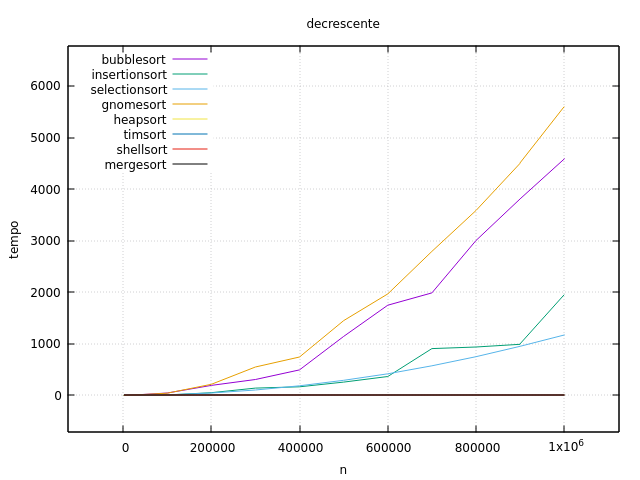
\includegraphics[width=0.8\textwidth]{graphs/decrescente-tempo.png}

Na Figura 4, os algorimos que levaram mais tempo para executar entradas maiores foram o bubblesort, insertionsort, selectionsort e gnomesort. Os demais algoritmos não levaram nem sequer 1 segundo para executar instâncias de $1\times10^6$.

\end{figure}

\begin{figure}[h]
\centering
\caption{Decrescente, N x Comparações}
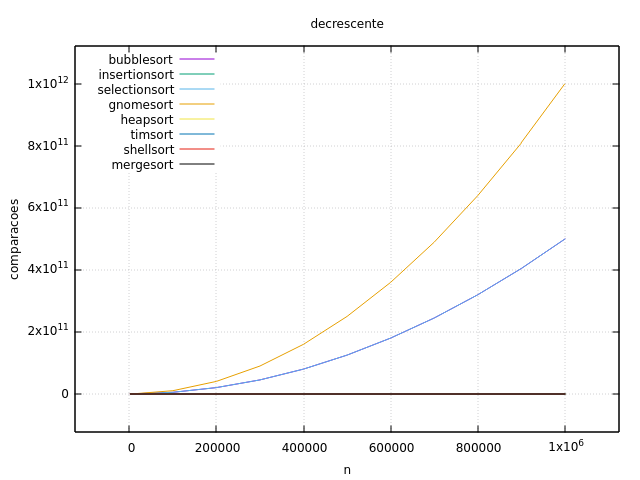
\includegraphics[width=0.8\textwidth]{graphs/decrescente-comparações.png}
\end{figure}

\begin{figure}[h]
\centering
\caption{Decrescente, N x Trocas}
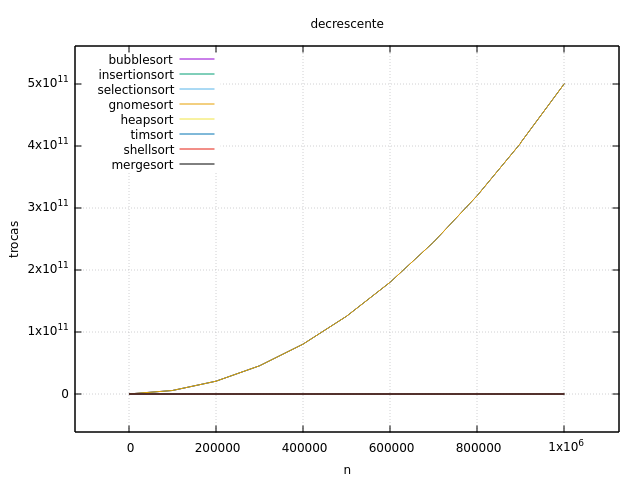
\includegraphics[width=0.8\textwidth]{graphs/decrescente-trocas.png}

Como é possível ver na Figura 6, os algoritmos que realizaram mais trocas foram o bubble, insertion e gnome. Os demais tiveram um quantidade de trocas significativas, mas, comparado aos anteriores, eles realizaram bem poucas, quase linear à quantide de elementos.
\end{figure}


\begin{figure}[h]
\centering
\caption{Crescente, N x Tempo}
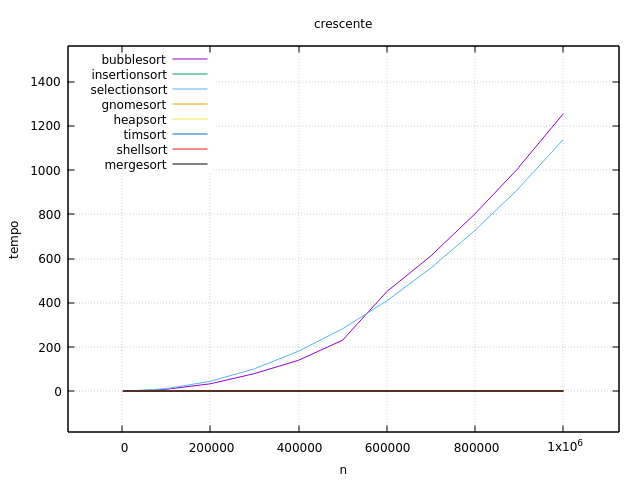
\includegraphics[width=0.8\textwidth]{graphs/crescente-tempo.png}

Na Figura 7, apesar do vetor já está ordenado, alguns algoritmos levaram um tempo considerável só para verificar o estado do vetor, como foram os casos do bubblesort e do selectionsort. Os demais algorimos não levaram nem 1 segundo para processar vetores ordenados de $1\times10^6$. Isso se dá ao fato que tanto o bubble quanto o selection sort verificam todos os elementos do vetor para cada elemento, na busca de colocá-lo na lugar correto.

\end{figure}

\begin{figure}[h]
\centering
\caption{Crescente, N x Comparações}
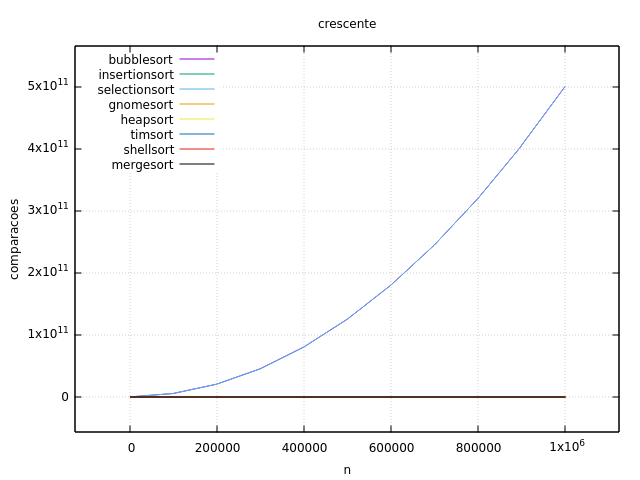
\includegraphics[width=0.8\textwidth]{graphs/crescente-comparações.png}

Já na Figura 8, os algorimtos que mais realizaram comparações em um vetor ordenado foram o bubble e selection sort. Novamente, como foi dito, esses algorimtos verificam todos os elementos do vetor para cada elemento, na busca de colocá-lo na lugar correto.

\end{figure}

\section{Considerações}

\backmatter 
\singlespacing   
% ----------------------------------------------------------------------------------------------------- %
\bibliography{relatorio_exemplo}

\appendix
\onehalfspacing
\end{document}